\chapter{Grundlagen}

\section{Projektumfeld}

Das Projekt wird im Umfeld der \gls{DHBW} Karlsruhe durchgeführt.

\section{Funktionsweise WLAN}

\subsection{SSID}

\subsection{BSSID}

\subsection{Signalstärke RSSI}

\section{Beispiel eines Workflows}

In folgender \autoref{fig:beschaffungsverfahren} ist ein Beispiel für einen Prozess an der \gls{DHBW} Karlsruhe dargestellt.
Es ist das \enquote{Beschaffungs-Genehmigungsverfahren}, das benötigt wird, um eine Bestellung für die \gls{DHBW} durchzuführen.

\begin{figure}
	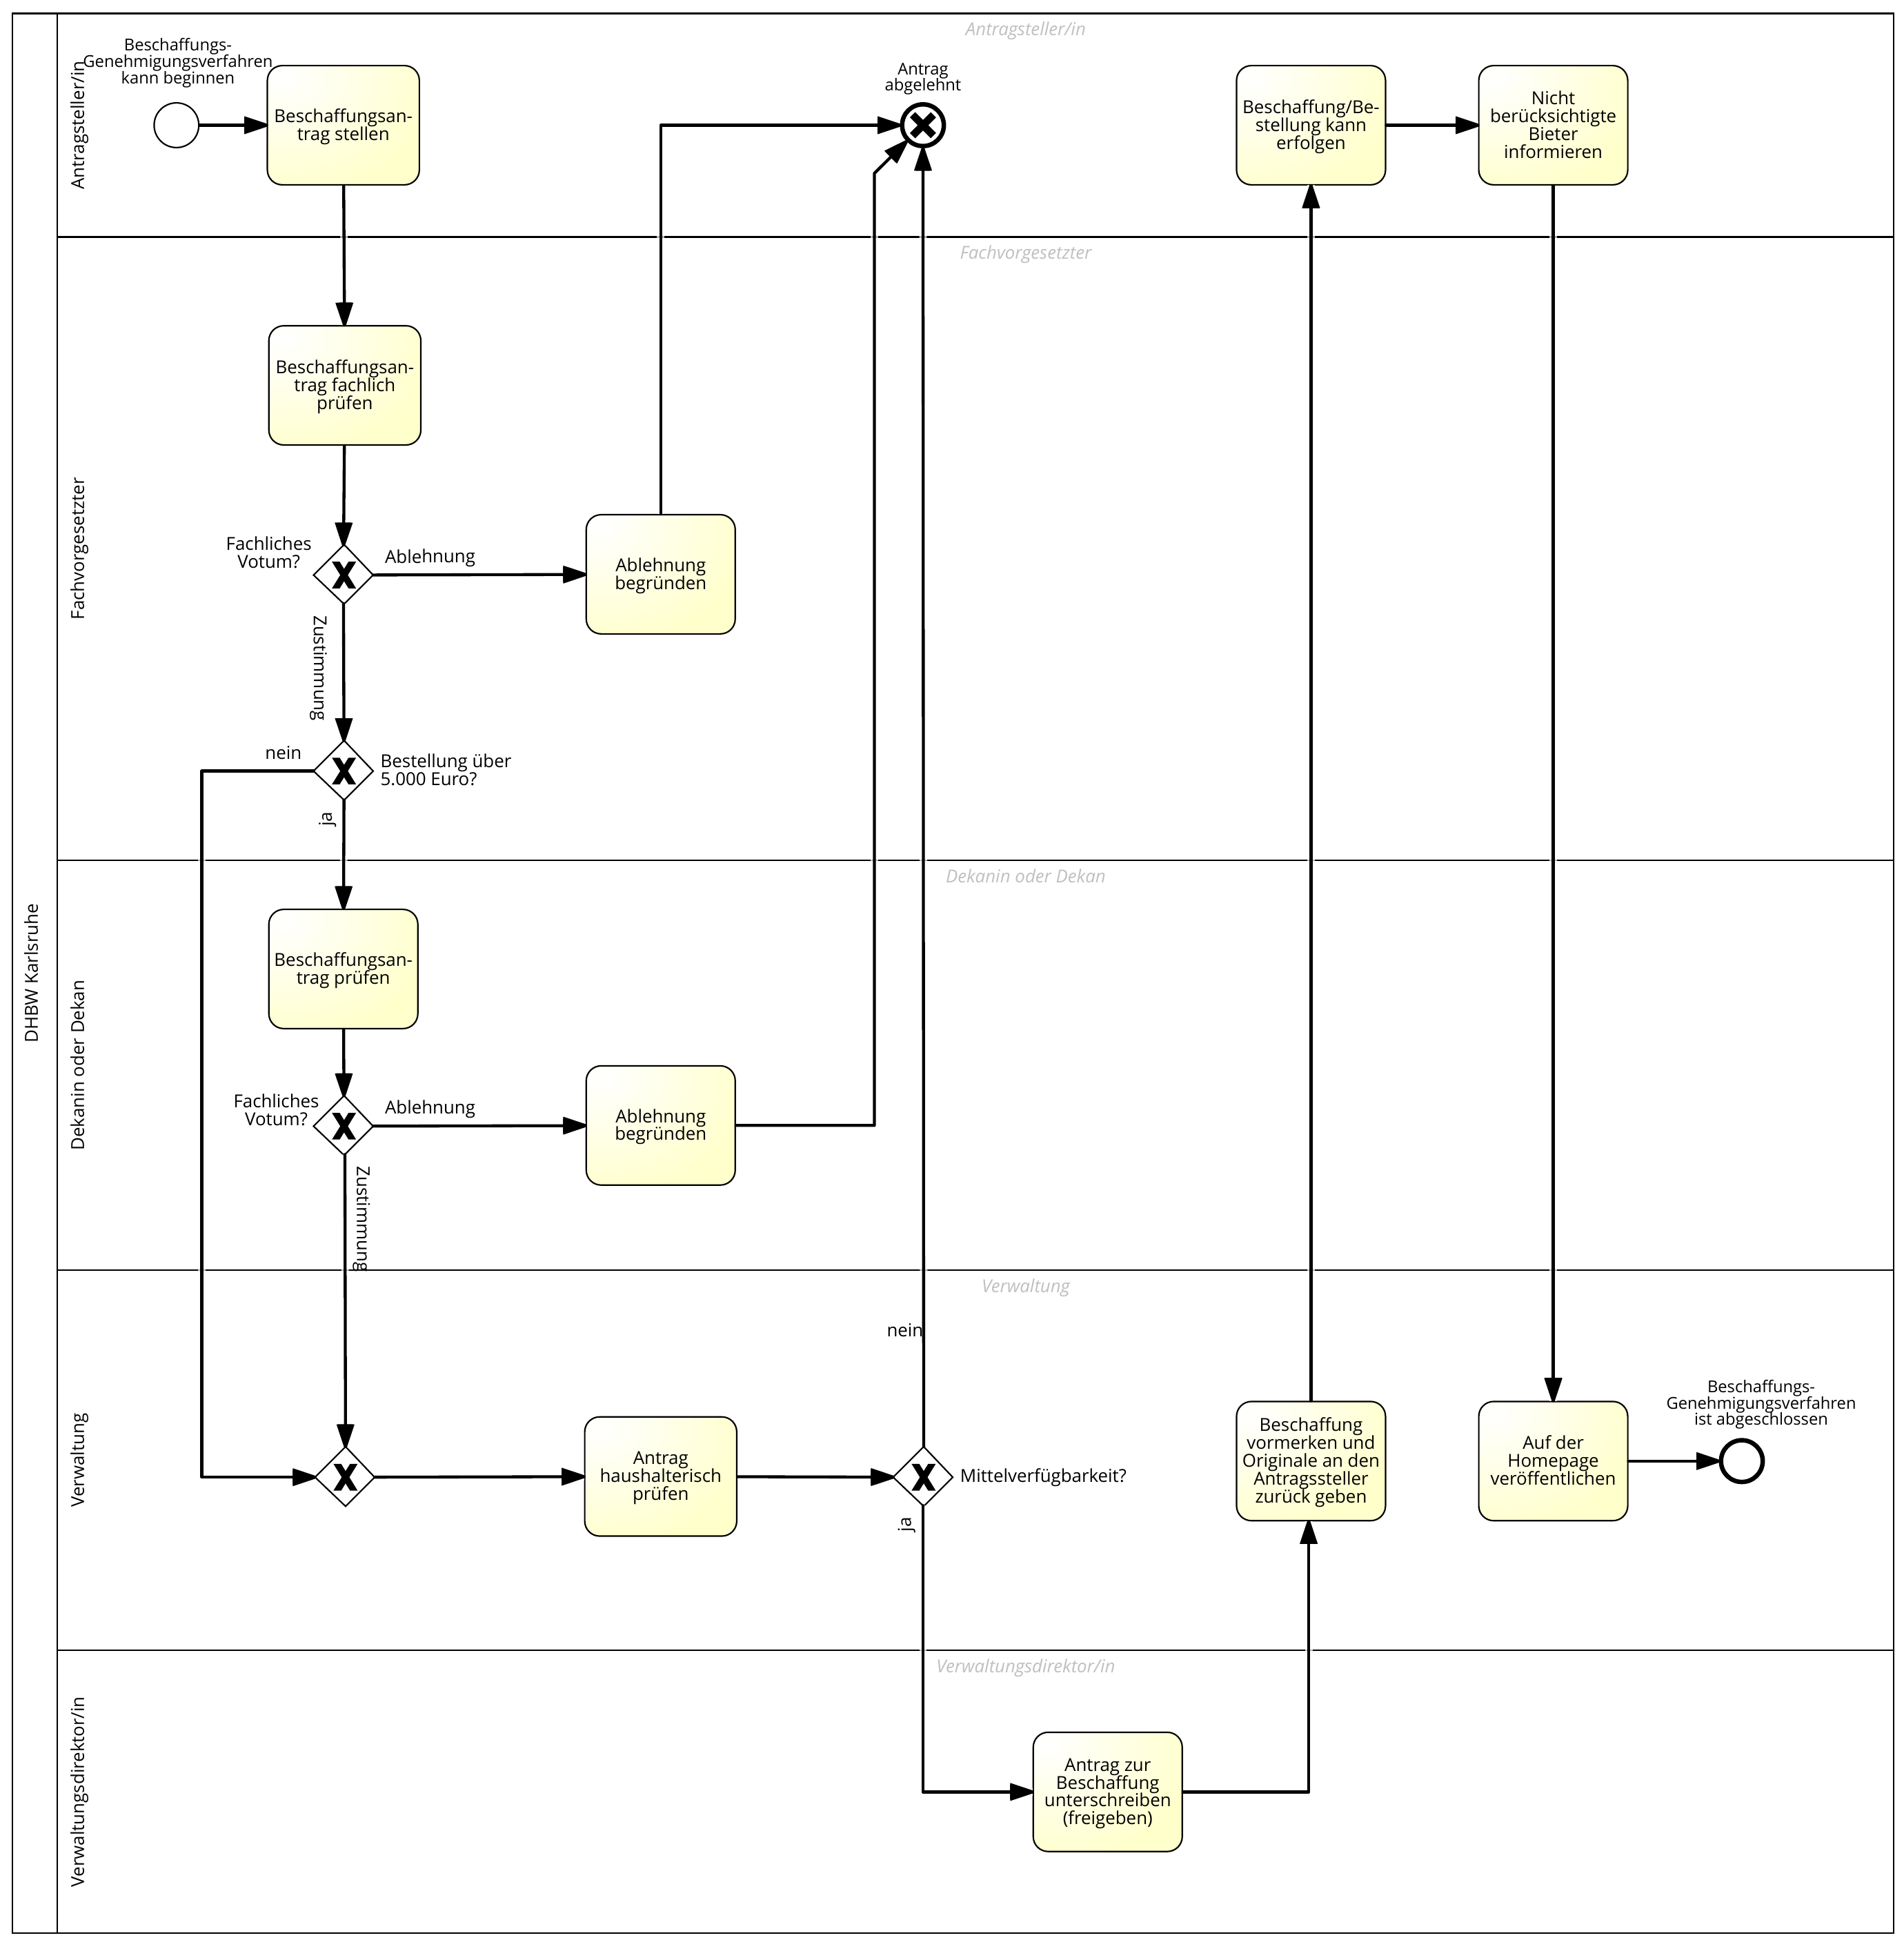
\includegraphics[width=\textwidth]{images/beschaffungs-genehmigungsverfahren.png} 
	\centering
	\caption{Beschaffungs-Genehmigungsverfahren der \gls{DHBW}}
	\label{fig:beschaffungsverfahren}
\end{figure} 

Der Prozess beginnt mit dem Antragsteller, welcher den Beschaffungsantrag stellt.
Der Antrag geht zum Fachvorgesetzten des Antragsteller, welcher diesen fachlich prüft.
Ist die Prüfung nicht erfolgreich, wird eine Ablehnung begründet und der Prozess beendet.

Bei erfolgreicher Prüfung muss der Antrag, wenn er über 5.000€ liegt, zudem vom Dekan geprüft werden.
Dieser kann entweder den Antrag wie oben beschrieben ablehnen oder stimmt diesem zu.

Ist der Antrag für eine Bestellung unter 5.000€ oder er bekommt die Zustimmung des Dekans, erhält als nächstes die Verwaltung den Antrag.
Die Verwaltung muss prüfen, ob die Mittel für diese Bestellung vorhanden sind.
Sind die Mittel nicht vorhanden, wird der Antrag abgelehnt.
Bei vorhandenen Mitteln wird der Antag von dem Verwaltungsdirektor unterschrieben und damit freigegeben.
Damit wird die Beschaffung in der Verwaltung vorgemerkt und der Antrag geht an den ursprünglichen Antragsteller zurück.

Sobald der Antragsteller den unterzeichneten Antrag erhält, kann die Beschaffung erfolgen.
In diesem Schritt müssen mögliche nicht berücksichtigte Bieter im Falle einer Ausschreibung informiert werden.

Im letzten Schritt veröffentlicht die Verwaltung das Ergebnis der Beschaffung auf der Homepage und der Prozess ist erfolgreich abgeschlossen.
